% Following command is used to create grouped signature line for Four Authors
\newcommand*\wildcard[2][6cm]{\vspace{1cm}\parbox{#1}{\hrulefill\par#2}} 

% A "parbox{}{}" is a box whose contents are created in paragraph mode. 
% "hrulefill{} to change thickness of underline"

\section*{Declaration}

It is hereby declared that

\begin{enumerate} % begin{enumerate} function to create numbered list
  \item The thesis submitted is my/our own original work while completing degree at Brac University.
  \item The thesis does not contain material previously published or written by a third party, except where this is appropriately cited through full and accurate referencing.
  \item The thesis does not contain material which has been accepted, or submitted, for any other degree or diploma at a university or other institution.
  \item We have acknowledged all main sources of help.
\end{enumerate}

\vspace{1cm}
\textbf{Student’s Full Name \& Signature:} % Testbf{} for Bold
\vspace{.5cm}

% CROP the signatures with minimum height possible. The width will always be resized to 6cm.
\begin{center}
    \begin{tabular}[b]{@{} p{6cm} @{}}
        
\includegraphics[width=6cm]{images/signatures/tahmid.jpg} \\
        \hline
        \centerline{\studentonename}
        \centerline{\studentoneid}
    \end{tabular}
    % Remove the following 7 lines if there's no second author.
    \hspace{2.5cm} %horizontal space added to create a gap between the two signatures in the same line
    \begin{tabular}[b]{@{} p{6cm} @{}}
        
\includegraphics[width=6cm]{images/signatures/emon.jpg} \\
        \hline
        \centerline{\studenttwoname}
        \centerline{\studenttwoid}
    \end{tabular} \\ %this double backslash is to create a new signature in the next line
    % Remove the following 6 lines if there's no third author.
    \begin{tabular}[b]{@{} p{6cm} @{}}
        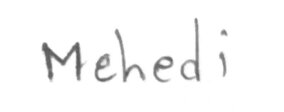
\includegraphics[width=6cm]{images/signatures/Mehedi.jpg} \\
        \hline
        \centerline{\studentthreename}
        \centerline{\studentthreeid}
    \end{tabular}
    % Remove the following 7 lines if there's no fourth author.
    \hspace{2.5cm}
    \begin{tabular}[b]{@{} p{6cm} @{}}
        
\includegraphics[width=6cm]{images/signatures/nuclear.jpg} \\
        \hline
        \centerline{\studentfourname}
        \centerline{\studentfourid}
    \end{tabular} \\
    % Remove the following 6 lines if there's no fifth author.
 
\end{center}


\pagebreak





